% Title: OR gate
% Author: Ramón Jaramillo.
\documentclass[tikz,border=10pt]{standalone}
%%%<
\usepackage{verbatim}
%%%>
\begin{comment}
:Title: One of the Quad-2 inputs OR Gate in MC14071B
:Tags: Circuitikz;Electrical engineering
:Author: Ramón Jaramillo
:Slug: or-gate

This circuit diagram depicts a network of PMOS and NMOS transistors that 
represents one of the Quad-2 inputs OR Gate in the MC14071B IC, based on 
these transistors. This schema was taken from a handbook online of
ON Semiconductors. Improvements and additions to this diagram are welcome.

Source: http://www.onsemi.com/pub_link/Collateral/MC14001B-D.PDF
\end{comment}
\usepackage[siunitx]{circuitikz}
\begin{document}
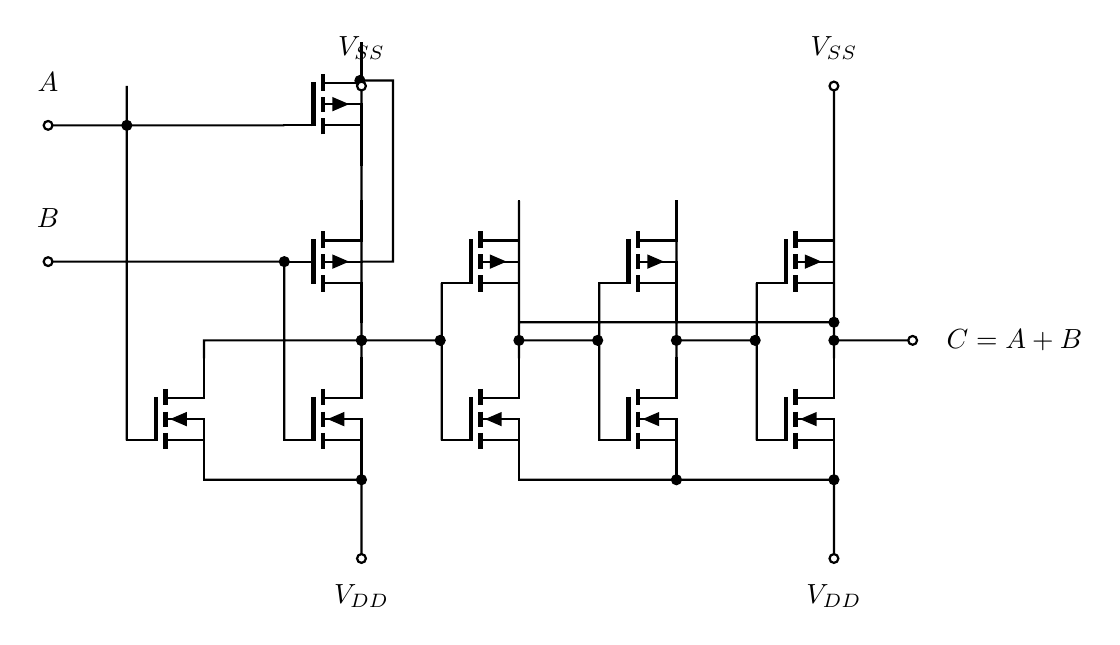
\begin{tikzpicture}[scale=2] 
  \draw[color=black, thick]
  % Name of MOSFET transistors left to right
  % Left to right in baseline: nmos1, nmos2, nmos3, nmo4 & nmos5.
  % Drawing the transistor and nodes using relative coordinates
    (0,0) node[nigfete] (nmos1) {}
    (1,0) node[nigfete] (nmos2) {}
    (nmos1.S) to (nmos2.S)
    % Connections to V_DD
    to [short,*-o] ++(0,-0.5) {} node[below=2mm] {$V_{DD}$}
    (1,1) node[pfet,yscale=-1] (pmos1) {} % yscale=-1 is mandatory to drawing
    % MOSFETs with the right sense.
    (1,2) node[pigfete,yscale=-1] (pmos2) {}
    (nmos2.G) to [short,-*] (pmos1.G)
    (pmos1.D) to (nmos2.D)	
    (nmos1.G) -- ++(0,1.5) -- ++(0,0.75)
    (pmos2.G) to [short,-*] ++(-1,0){}
    to [short,-o] ++(-0.5,0) {} node[above=3mm] {$A$}
    (pmos1.G) to [short,-o] ++(-1.5,0) {} node[above=3mm] {$B$}
    (pmos1.B) -- ++(0.2,0) -| ++(0,1.15) to [short,-*]++(-0.21,0)
    (pmos1.S) -- (pmos2.D) {}
    % Inverter
    (2,0) node[nigfete](nmos3) {}
    (2,1) node[pigfete, yscale=-1] (pmos3) {}
    (nmos3.G) to (pmos3.G)
    (nmos3.D) to (pmos3.D)
    % Gate OR Output
    (3,0) node[nigfete](nmos4){}
    (3,1) node[pigfete, yscale=-1] (pmos4) {}
    (nmos4.G) to (pmos4.G)
    (nmos4.D) to (pmos4.D)
    %%%
    (4,0) node[nigfete] (nmos5) {}
    (4,1) node[pigfete, yscale=-1] (pmos5) {}
    (nmos5.G) to (pmos5.G)
    (nmos5.D) to (pmos5.D)
    % Connection to V_DD
    (nmos3.S) to [short,-*] (nmos4.S) -- (nmos5.S)
    to [short,*-o] ++(0,-0.5) {} node[below=2mm] {$V_{DD}$}
    % Connection to V_DD
    (pmos3.S) -- (pmos4.S) -- (pmos5.S)
    to [short,*-o] ++(0,1.5) {} node[above=2mm] {$V_{SS}$}
    (pmos2.S) to [short,-o] ++(0,0.5) {} node[above=2mm] {$V_{SS}$}
    %(3,-0.4) node[circ] {}
    % Connections between nodes
    (nmos1.D) -| (0,0.5) to [short,-o] (1,0.5) {}
    (1,0.5) to  [short,*-*] ++(0.5,0) {}
    (2,0.5) to  [short,*-*] ++(0.5,0) {}
    (3,0.5) to  [short,*-*] ++(0.5,0) {}
    (4,0.5) to  [short,*-o] ++(0.5,0) {} node[right=3mm] {$C=A+B$}
  ;
\end{tikzpicture}
\end{document}